\section{Résultats}\label{sec:resultats}
Les résultats sont divisés en trois parties : les mesures que l'on a prises ainsi que les constantes
utilisées ;
les calculs effectués afin d'obtenir $\eta $ et finalement les simulations faites de la valeur
de $\eta $.
Toute l'exploitation de ces résultats sera faite dans la section suivante (cf.
section~\ref{sec:analyse-des-resultats}).

\subsection{Mesures}\label{subsec:mesures}
Premièrement, voici les constantes et autres données dont nous avons besoin :
l'accélération terrestre $g= 9.81 \left[ \frac{m}{s^{2}} \right] $, la masse volumique de l'acier
($\rho_{acier} = 7850 \left[ \frac{Kg}{m^{3}} \right] $) et la masse volumique de la glycérine
($\rho_{glycérine} = 1260 \left[ \frac{Kg}{m^{3}} \right] $).
De plus, les trois diamètres différents des billes sont 1, $1.5$ et 2 $[mm]$ soit
$1\cdot 10^{-3}$, $1.5\cdot 10^{-3}$ et $2\cdot 10^{-3}$ $[m]$.
De fait, leurs rayons sont :
\begin{table}[H]
    \centering
    \begin{tabular}{|>{\columncolor{darkgray}} l||l|>{\columncolor{gray}} l|l|}
        \hline
        Diamètre [mm] & 1 & 1.5 & 2 \\
        \hline
        Rayon [m] & $5 \cdot 10^{-4}$ & $7.5\cdot 10^{-4}$ & $1 \cdot 10^{-3}$\\
        \hline
    \end{tabular}
    \caption{Rayon des billes à partir de leur diamètre}
    \label{tab:raybille}
\end{table}
Ensuite, le temps que mets chaque une des billes pour parcourir la distance de $8.5 [cm] = 8.5 \cdot
10^{-2} [m]$ dans la glycérine, mesures réitérées 5 fois par bille :
\begin{table}[H]
    \centering
    \begin{tabular}{|>{\columncolor{darkgray}} l||l|>{\columncolor{gray}} l|l|>{\columncolor{gray}} l|l|}
        \hline
        \rowcolor{darkgray} \cellcolor{black} & $t_{1} [s]$ & $t_{2} [s]$ & $t_{3} [s]$ & $t_{4} [s]$ & $t_{5} [s]$\\
        \hline \hline
        D = 1 [mm] & 4.07 & 4.15 & 4.11 & 4.05 & 4.18\\
        \hline
        D = 1.5 [mm] & 1.63 & 1.83 & 1.74 & 1.88 & 1.77\\
        \hline
        D = 2 [mm] & 1.15 & 1.14 & 1.17 & 1.18 & 1.14\\
        \hline
    \end{tabular}
    \caption{Temps de descente mesuré de chaque bille}
    \label{tab:temps-mesure}
\end{table}

\subsection{Calculs}\label{subsec:calculs}
Pour chaque bille, on a pris la moyenne des temps afin de calculer $\eta$ :
\begin{table}[H]
    \centering
    \begin{tabular}{|>{\columncolor{darkgray}} l||l|>{\columncolor{gray}} l|l|}
        \hline
        Diamètre [mm] & 1 & 1.5 & 2 \\
        \hline
        T [s] & 4.112 & 1.770 & 1.156 \\
        \hline
    \end{tabular}
    \caption{Temps moyens de chute des billes}
    \label{tab:meantime}
\end{table}
Ensuite, on calcule la vitesse de la bille (avec $v= \frac{d}{t} $):
\begin{table}[H]
    \centering
    \begin{tabular}{|>{\columncolor{darkgray}} l||l|>{\columncolor{gray}} l|l|}
        \hline
        Diamètre [mm] & 1 & 1.5 & 2 \\
        \hline
        Vitesse $\left[ \frac{m}{s} \right] $ & $2.067 \cdot 10^{-2}$ & $4.802\cdot 10^{-2}$ & $7.353 \cdot 10^{-2}$\\
        \hline
    \end{tabular}
    \caption{Vitesse des billes selon de leur diamètre}
    \label{tab:vitesse}
\end{table}
Finalement, on calcule $\eta$ avec la formule expliquée dans l'introduction $\eta = \frac{2 R^{2} g (\rho_{acier} - \rho_{glycérine})}
{9 v} $ :
\begin{table}[H]
    \centering
    \begin{tabular}{|>{\columncolor{darkgray}} l||l|>{\columncolor{gray}} l|l|}
        \hline
        Diamètre [mm] & 1 & 1.5 & 2 \\
        \hline
        $\eta$ $[mPs \cdot s ]$ & $173.75$ & $168.27$ & $195.38$\\
        \hline
    \end{tabular}
    \caption{$\eta$ pour chaque bille}
    \label{tab:eta-val}
\end{table}
Donc si l'on prend la moyenne comme valeur pour la suite : $\eta_{moy} \approx 179.13 [mPa \cdot s] $.

\subsection{Simulations}\label{subsec:simulations}
Avec la valeur de $\eta$ obtenue, et en se servant de la somme des forces évoquée en introduction
lorsque la vitesse n'est pas constante $F_{p}-F_{a}-F_{f}=m \cdot a$, on va faire des simulations
de l'évolution de la vitesse en fonction du temps selon le rayon de la bille et de la vitesse
initiale ($v_{0}$).
\subsubsection{Itératives}
Première méthode pour faire ces simulations : prendre un interval de temps, calculer la vitesse en
$t_{i+1}$ avec l'accélération en $t$ via un MRUA ($v(t) = v_{0} + a \cdot t $) et l'accélération
en $t_{i+1}$ via la vitesse précédement calculée par la somme des forces
$\frac{4}{3}\pi R^{3} \cdot \rho_{acier} \cdot g - \rho_{glycérine} \cdot \frac{4}{3}\pi R^{3}
\cdot g - 6 \pi R \cdot \eta \cdot v =  \frac{4}{3}\pi R^{3} \cdot \rho_{acier} \cdot a \Longleftrightarrow a =
\frac{g (\rho_{acier}-\rho_{glycérine})}{\rho_{acier}} - \frac{9 \eta }{2 R_{2} \rho_{acier}}\cdot v
= A - B \cdot v $ (les grosses valeurs constantes ont été substituées par A et B ; sur les graphes,
on nomme les courbes selon leur $v_{0}$).
\begin{minipage}{0.475\textwidth}
    \begin{figure}[H]
        \centering
        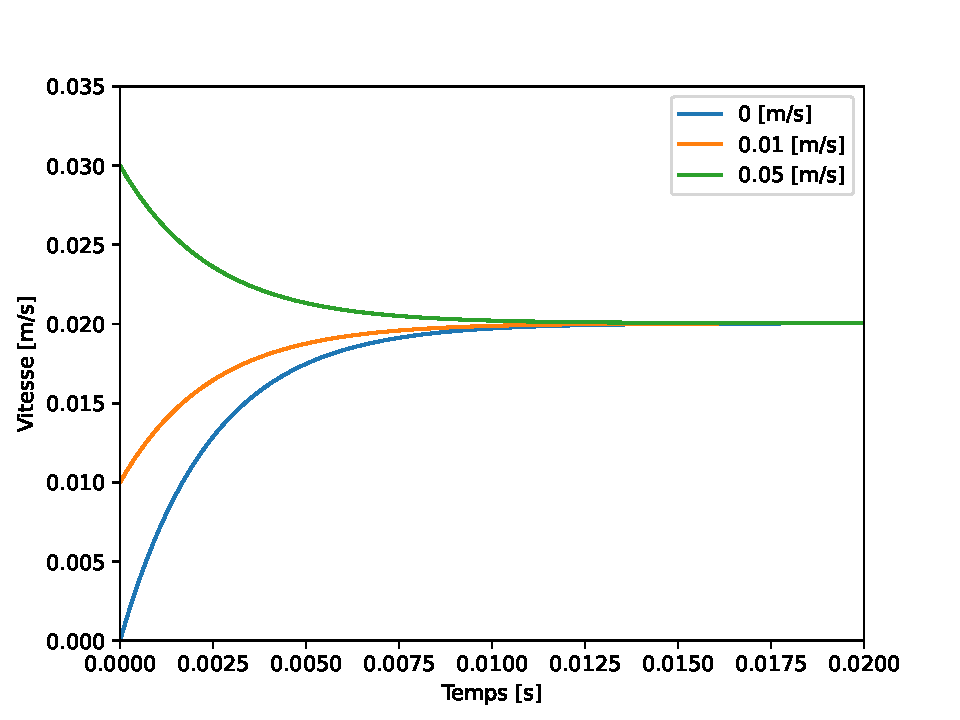
\includegraphics[scale=0.55]{graph/ray1_it}
        \caption{Vitesse pour une bille de 1 [mm] de diamètre}
        \label{fig:ray1_it}
    \end{figure}
\end{minipage}
\begin{minipage}{0.05\textwidth}
\end{minipage}
\begin{minipage}{0.475\textwidth}
    \begin{figure}[H]
        \centering
        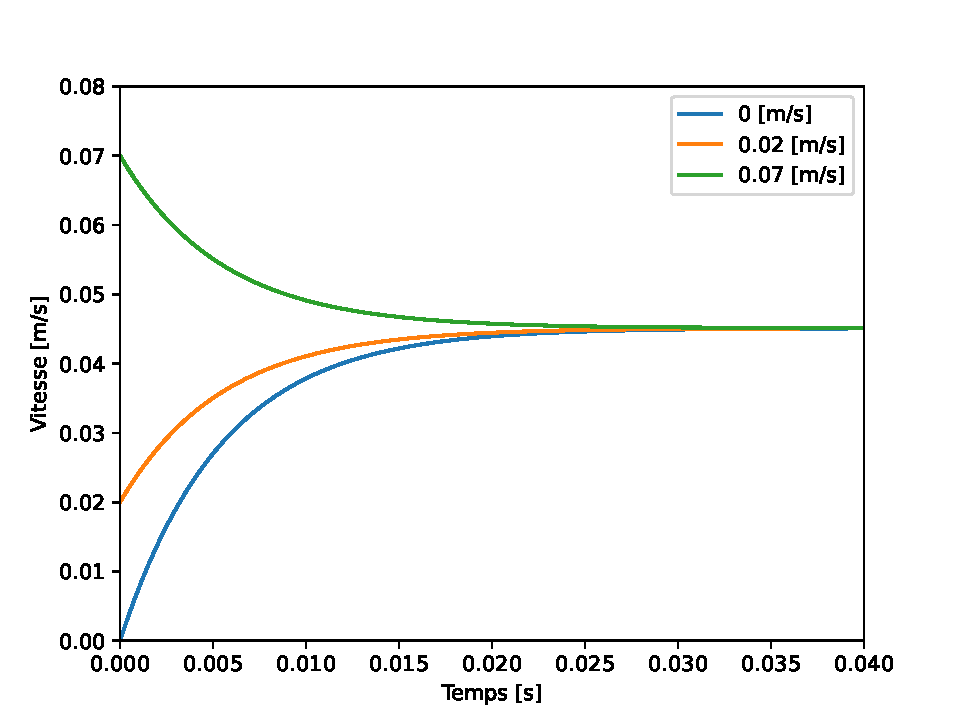
\includegraphics[scale=0.55]{graph/ray2_it}
        \caption{Vitesse pour une bille de 1.5 [mm] de diamètre}
        \label{fig:ray2_it}
    \end{figure}
\end{minipage}
\begin{figure}[H]
    \centering
    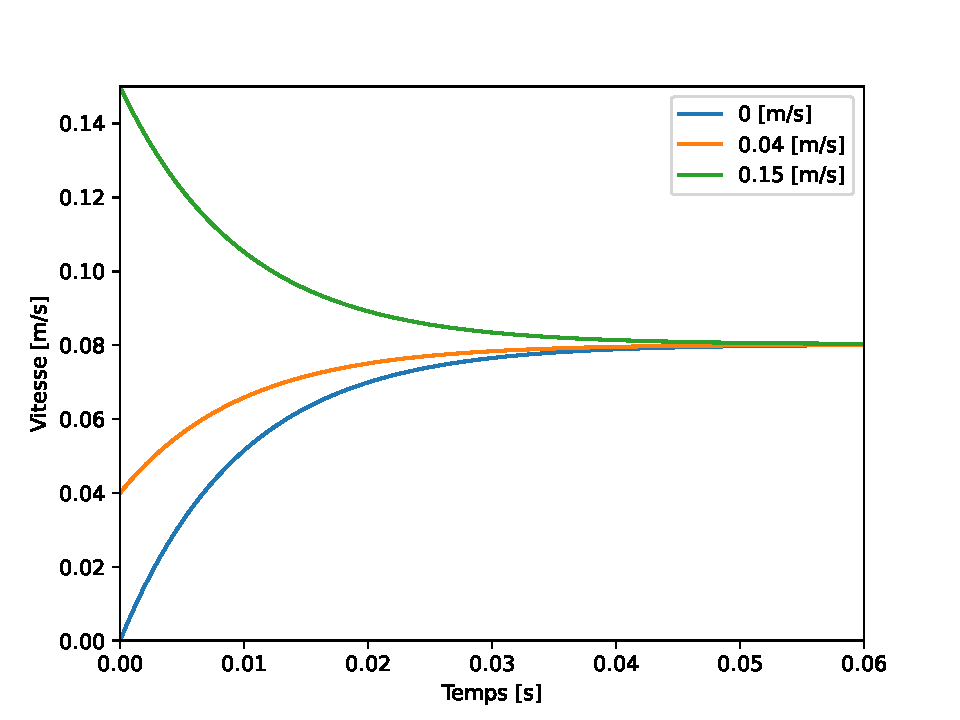
\includegraphics[scale=0.55]{graph/ray3_it}
    \caption{Vitesse pour une bille de 2 [mm] de diamètre}
    \label{fig:ray3_it}
\end{figure}

\subsubsection{Autres}
Comme autre méthode, on peut résoudre mathématiquement l'équation différentielle \footnote{Note :
la résolution d'équation différentielle est faite via "Wolfram Alpha" car on ne maitrise pas très
bien ces outils. Néanmoins, les dérivées et intégrales en section~\ref{sec:analyse-des-resultats} sont juste
verifiée avec ce logiciel.} $a(t)= v'(t) = A - B \cdot v(t) \Longleftrightarrow v(t) = \frac{A}{B}+c \cdot
e^{-B\cdot t} $ où $c$ est une constante que l'on peut calculer vu que l'on connait $v_{0}$
($t=0$, donc $v_{0} = \frac{A}{B}+c \Longleftrightarrow c = v_{0}- \frac{A}{B}$)[cf.\ figure~\ref{fig:ray3_th}].\\
En prenant beaucoup de valeurs $v_{0}$ de départ, on peut également faire une image de la densité de
points qui illustre bien la convergence de la vitesse en une limite [cf.\ figure~\ref{fig:densplot}].\\
\begin{minipage}{0.475\textwidth}
    \begin{figure}[H]
        \centering
        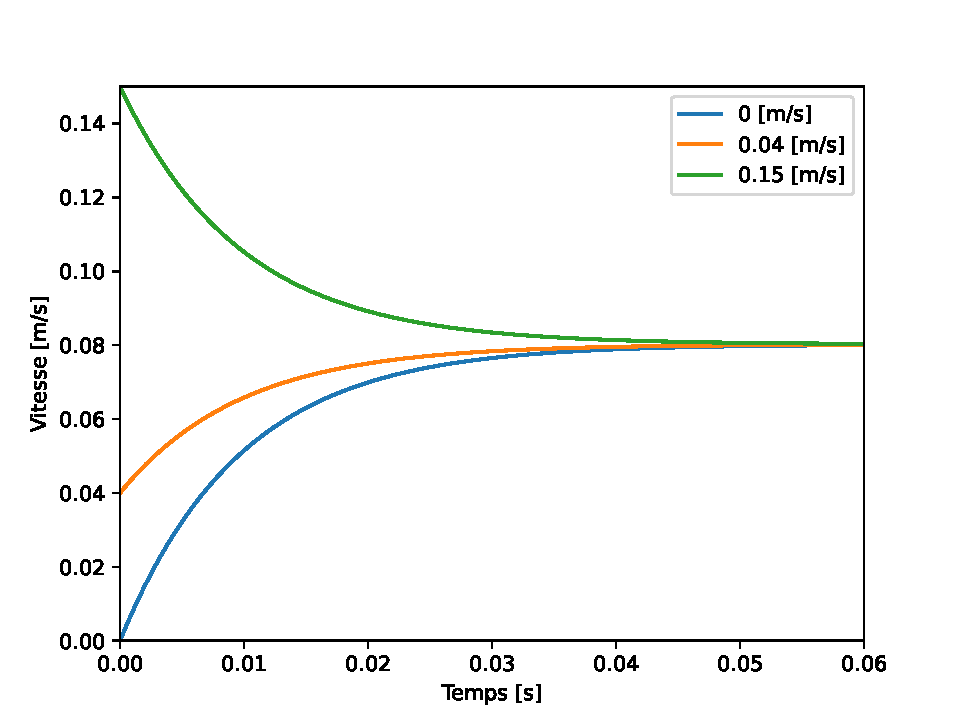
\includegraphics[scale=0.54]{graph/ray3_th}
        \caption{Vitesse pour une bille de 2 [mm] de diamètre avec la fonction théorique}
        \label{fig:ray3_th}
    \end{figure}
\end{minipage}
\begin{minipage}{0.05\textwidth}
\end{minipage}
\begin{minipage}{0.475\textwidth}
    \begin{figure}[H]
        \centering
        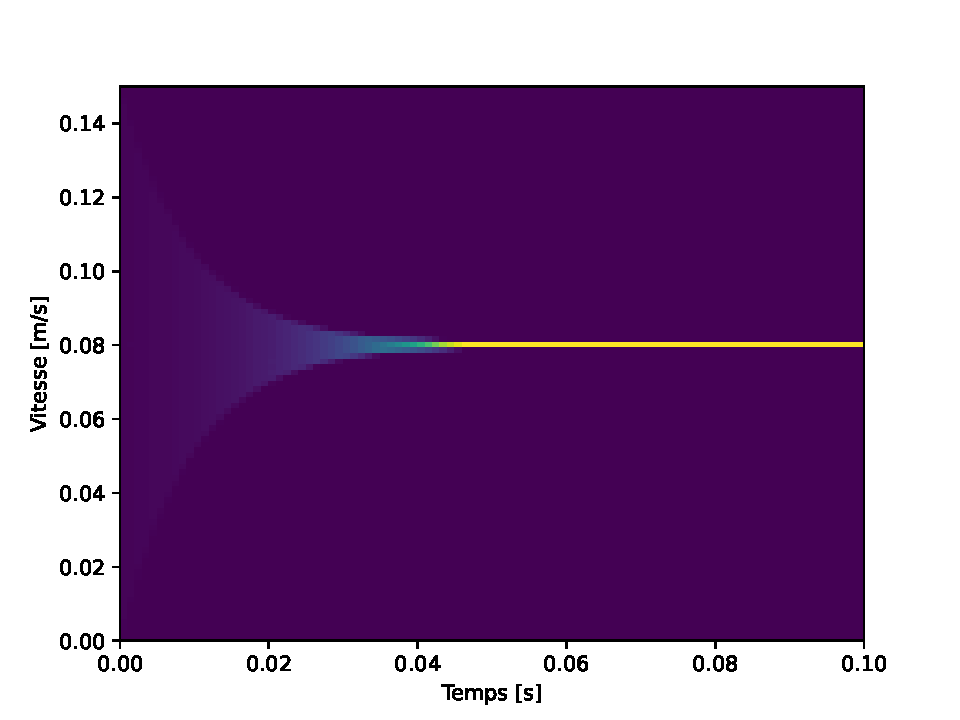
\includegraphics[scale=0.54]{graph/densplot}
        \caption{"Densité" de la vitesse en fonction du temps pour une bille de 2 [mm] de diamètre}
        \label{fig:densplot}
    \end{figure}
\end{minipage}
